\subsection{Recovery Protocols}
\label{proto_reco}

The \dcamp Recovery Protocols are used for the \hyperref[algor_promo]{Promotion} and \hyperref[algor_elect]{Election}
algorithms and use the same base messages as the \hyperref[proto_topo]{Topology Protocol}, \texttt{TOPO} and
\texttt{CONTROL}.

\begin{figure}[H]
\vspace{+10pt}
\begin{verbatim}
branch-recovery  = *sos group-stop
sos              = B-SOS R-KEEPCALM
group-stop       = R-GROUP B-POLO R-STOP
\end{verbatim}
\vspace{-5pt}
\caption[Branch Recovery Protocol]
	{Branch Recovery Protocol: \texttt{R-} represents the Root node sending a message and \texttt{B-} represents a
	 Base node sending a message.}
\label{fig:proto_reco_branch_spec}
\end{figure}

The Branch Recovery Protocol is initiated by Base nodes when they detect their Collector has died. Once the Root node
has received an \texttt{SOS} message from at least one third of the branch's Base nodes, the Root proceeds to shutdown
the entire branch using the Topology Protocol.

\begin{figure}[H]
    \centering
    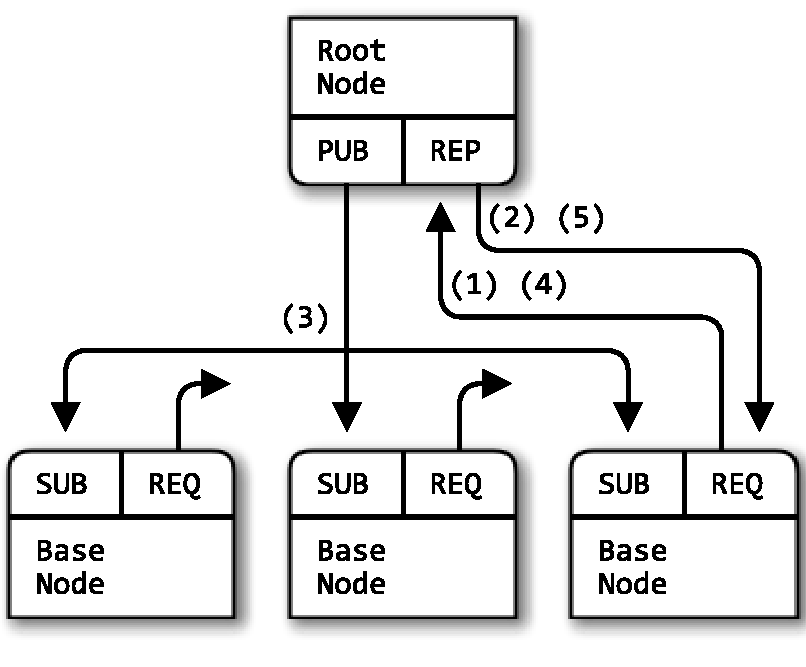
\includegraphics[scale=0.5]{branch-recovery.pdf}
    \label{fig:proto_branch_reco_image}
    \caption[Branch Recovery Protocol Diagram]
            {Branch Recovery Protocol Diagram: (1) \texttt{SOS}, (2) \texttt{KEEPCALM}, (3) \texttt{GROUP}, (4)
	    \texttt{POLO}, (5) \texttt{STOP}}
\end{figure}

\texttt{SOS} and \texttt{KEEPCALM} are shorthand for the \texttt{CONTROL} message with a command value of \texttt{"sos"}
and \texttt{"keepcalm"} respectively. The \texttt{POLO} and \texttt{STOP} messages come directly from the Topology
Protocol.

The \texttt{GROUP} message is similarly shorthand for the \texttt{TOPO} message with a key value of
\texttt{"/GROUP/<group-name>"}. This takes advantage of ZeroMQ's Pub-Sub filtering to only stop the faulty branch.

\begin{figure}[H]
\vspace{+10pt}
\begin{verbatim}
root-recovery  = *election
election       = C-WUTUP *C-YO C-IWIN
\end{verbatim}
\vspace{-5pt}
\caption[Root Recovery Protocol]
        {Root Recovery Protocol: \texttt{C-} represents a Collector node sending a message.}
\label{fig:proto_reco_root_spec}
\end{figure}

As each Collector node detects the Root node has died, it attempts to start an election via the \texttt{WUTUP} message.
Collector nodes with higher UUIDs will respond to the first Collector by sending the \texttt{YO} message. If no
\texttt{YO} messages are received by the first Collector, the \texttt{IWIN} message is sent out to all Collector nodes,
self-declaring the first Collector as the new Root.

\begin{figure}[H]
    \centering
    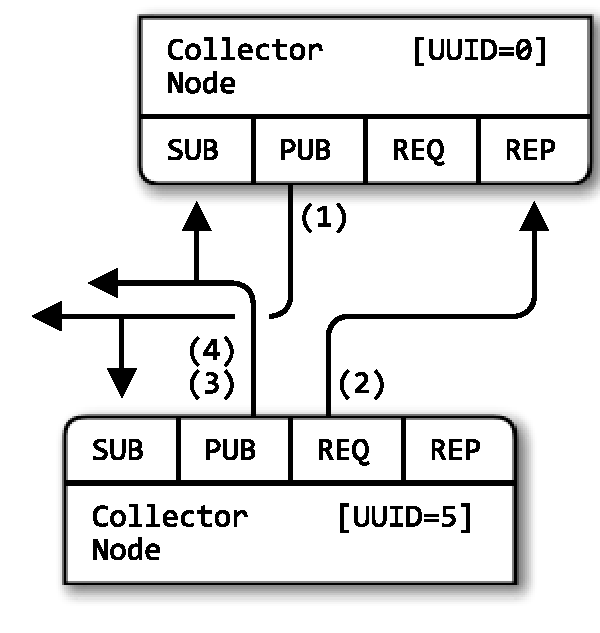
\includegraphics[scale=0.5]{root-recovery.pdf}
    \label{fig:proto_root_reco_image}
    \caption[Root Recovery Protocol Diagram]
	    {Root Recovery Protocol Diagram: (1) \texttt{WUTUP}, (2) \texttt{YO}, (3) \texttt{WUTUP}, (4) \texttt{IWIN}}
\end{figure}

The \texttt{WUTUP} and \texttt{IWIN} messages are shorthand for \texttt{TOPO(key="/RECOVERY/wutup"} and
\texttt{TOPO(key="/RECOVERY/iwin"} respectively. The \texttt{YO} message is shorthand for
\texttt{CONTROL(command="yo")}.
